\chapter{Results}
\label{ch:results}

This chapter reports the experiments defined in
\Cref{sec:method-coinflip}. \Cref{sec:results-setup} recaps the
setup and how to read the tables. \Cref{sec:results-baseline} shows
how vulnerable the unfiltered honeyword generators are to the CNN
attacker of \Cref{sec:method-cnn}. \Cref{sec:results-filter} isolates
the effect of the two-stage filter of \Cref{sec:method-filter} on
$\mathrm{ASR}@t$ and on the flatness criteria of
\Cref{sec:method-formalism}. \Cref{sec:results-cost} reports the
acceptance rates and regeneration counts and develops the
deployability-first reading of the results.
\Cref{sec:results-ntrain} confirms that the ordering
of methods is preserved across training-set sizes.
\Cref{sec:results-gan} isolates a distributional artifact of the GAN.
\Cref{sec:results-freq} evaluates the accepted sets against a
frequency attacker as a cross-attacker robustness check.
\Cref{sec:results-discussion} draws the picture together.

\section{Setup}
\label{sec:results-setup}

All experiments are run on the cleaned RockYou corpus. For each
training size $N_{\text{train}} \in \{2000,\,5000,\,10000\}$ a separate
oracle and generator are trained, and every trained generator produces
sweetword sets that are evaluated on a test set of $2000$ sweetword
sets (\Cref{sec:method-coinflip}). The attacker CNN is trained once on a
disjoint $5000$-password attacker corpus with HoneyGen-Baseline
negatives and reused unchanged across all training sizes and generators
(\Cref{sec:method-cnn}), so that a single, consistent adversary
evaluates every method. All parameter values are those of
\Cref{tab:params} in \Cref{sec:method-protocol}, i.e.\ the relaxed
thresholds adopted in \Cref{sec:method-threshold-tradeoff}.

The primary security metric is $\mathrm{ASR}@5$: the fraction of sets
on which the attacker's five highest-ranked guesses include the real
password. Under ideal flatness $\mathrm{ASR}@5 = 5/k = 0.25$ for
$k = 20$; higher values quantify how much better than random guessing
the attacker does. We also report the flatness criteria
$F_{\text{rank}}$ (the normalised rank of the real password; $0.5$ is
the ideal middle), $F_{\text{ent}}$ (normalised entropy of the induced
distribution; close to $1$ is uniform), and $F_{\varepsilon}$ (the
$\varepsilon$-flatness pass rate). \Cref{tab:params} lists every fixed
parameter. Unless stated otherwise, the detailed single-training-size
tables use $N_{\text{train}} = 10000$, the largest and most stable
corpus; \Cref{sec:results-ntrain} shows the smaller sizes reproduce
the same ordering.

% ===== Adopted parameter values =====
\begin{table}[t]
  \centering
  \begin{tabular}{llr}
    \toprule
    \textbf{Symbol} & \textbf{Meaning} & \textbf{Value} \\
    \midrule
    $k$ & Sweetword set size & 20 \\
    $\varepsilon_{\max}$ & $\varepsilon$-flatness bound ($q_{\max}\le 1/k+\varepsilon_{\max}$) & 0.05 \\
    $\delta_{H}$ & Entropy slack ($F_{\text{ent}}\ge 1-\delta_H$) & 0.10 \\
    $\text{gap}_{\max}$ & Top-gap threshold & 0.05 \\
    $\tau_{\text{band}}$ & Additive pre-screening band & 0.15 \\
    $\tau_{\text{band-ratio}}$ & Multiplicative pre-screening band & 2.0 \\
    $R_{\max}$ & Regeneration cap & 50 \\
    BS\_CNN & CNN training batch size & 256 \\
    Epochs (oracle / attacker) & CNN training epochs & 10 / 10 \\
    Epochs (GAN final / quick) & GAN training epochs & 60 / 20 \\
    Epochs (FastText final / quick) & FastText training epochs & 100 / 20 \\
    \bottomrule
  \end{tabular}
  \caption{Adopted parameter values for all experiments in \Cref{ch:results}.
  The flatness thresholds are the relaxed configuration of
  \Cref{sec:method-threshold-tradeoff}.}
  \label{tab:params}
\end{table}


\section{Unfiltered Baselines Under the CNN Attacker}
\label{sec:results-baseline}

The four unfiltered honeyword-generation strategies
(Chaffing-by-Tweaking, Chaffing-with-Password-Model,
Chaffing-with-Hybrid-Model, HoneyGen Baseline) are all highly
distinguishable to the CNN attacker. At $N_{\text{train}} = 10000$
they report $\mathrm{ASR}@5$ of 0.678, 0.755, 0.743, and 0.746
respectively (\Cref{tab:asr-master}), roughly three times the
random-guessing rate of $0.25$. Two points follow. First, the four
strategies cluster tightly: the three model-based generators are
within $0.02$ of one another, and the simplest rule-based generator,
Chaffing-by-Tweaking, is only about $0.07$ lower. Second, the more
elaborate statistical machinery of the hybrid and HoneyGen generators
does \emph{not} translate into flatness against a learned
discriminator: their $F_{\text{rank}}$ values sit near 0.169,
meaning the real password is ranked near the top of the twenty
candidates on the average set. This is the pattern that motivates the
filter.

\section{Effect of Flatness Filtering}
\label{sec:results-filter}

\Cref{tab:asr-master} reports $\mathrm{ASR}@1$, $\mathrm{ASR}@3$, and
$\mathrm{ASR}@5$ for all ten methods at the three training sizes, and
\Cref{tab:summary2000} consolidates the $N_{\text{train}} = 10000$
column with the flatness criteria and the filtering cost. Reading the
$\mathrm{ASR}@5$ column at $N_{\text{train}} = 10000$, the methods
separate into three families.

% ===== Master ASR table (CNN) =====
\begin{table}[t]
  \centering\small
  \setlength{\tabcolsep}{4pt}
  \begin{tabular}{lrrrrrrrrr}
    \toprule
    & \multicolumn{3}{c}{$N_{\text{train}}{=}2000$}
    & \multicolumn{3}{c}{$N_{\text{train}}{=}5000$}
    & \multicolumn{3}{c}{$N_{\text{train}}{=}10000$} \\
    \cmidrule(lr){2-4}\cmidrule(lr){5-7}\cmidrule(lr){8-10}
    \textbf{Method} & @1 & @3 & @5 & @1 & @3 & @5 & @1 & @3 & @5 \\
    \midrule
    Chaffing-by-Tweaking & 0.290 & 0.544 & 0.679 & 0.287 & 0.539 & 0.678 & 0.281 & 0.540 & 0.678 \\
    Chaffing-with-Password-Model & 0.303 & 0.615 & 0.759 & 0.300 & 0.617 & 0.767 & 0.304 & 0.600 & 0.755 \\
    Chaffing-with-Hybrid-Model & 0.341 & 0.611 & 0.756 & 0.338 & 0.620 & 0.752 & 0.337 & 0.603 & 0.743 \\
    HoneyGen Baseline & 0.339 & 0.614 & 0.752 & 0.336 & 0.619 & 0.761 & 0.346 & 0.604 & 0.746 \\
    \addlinespace
    HoneyGen + Set-Filter & 0.305 & 0.583 & 0.728 & 0.115 & 0.323 & 0.518 & 0.179 & 0.438 & 0.610 \\
    HoneyGen + Prescreen-Add & 0.164 & 0.412 & 0.588 & 0.109 & 0.299 & 0.470 & 0.144 & 0.368 & 0.525 \\
    HoneyGen + Prescreen-Ratio & 0.083 & 0.262 & 0.417 & 0.071 & 0.205 & 0.341 & 0.071 & 0.217 & 0.341 \\
    HoneyGen + Hybrid-Add & 0.222 & 0.473 & 0.641 & 0.093 & 0.299 & 0.462 & 0.141 & 0.364 & 0.510 \\
    HoneyGen + Hybrid-Ratio & 0.139 & 0.350 & 0.503 & 0.083 & 0.172 & 0.285 & 0.050 & 0.167 & 0.293 \\
        GAN (Self-Trained) & 0.101 & 0.222 & 0.331 & 0.565 & 0.718 & 0.774 & 0.745 & 0.832 & 0.872 \\
    \addlinespace
    Random guessing ($t/k$) & 0.050 & 0.150 & 0.250 & 0.050 & 0.150 & 0.250 & 0.050 & 0.150 & 0.250 \\
    \bottomrule
  \end{tabular}
  \caption{$\mathrm{ASR}@t$ under the CNN attacker for all ten methods at
    three training sizes, reported as the rational-attacker value of
  \Cref{eq:rational}; no entry falls below the random-guessing baseline
  $t/k$.
  Columns are $\mathrm{ASR}@1$, $\mathrm{ASR}@3$, $\mathrm{ASR}@5$.
  Each block is evaluated on a test set of sweetword sets produced by
  the generator trained at that $N_{\text{train}}$.}
  \label{tab:asr-master}
\end{table}


\paragraph{Unfiltered baselines.}
The four baselines occupy the vulnerable band, $\mathrm{ASR}@5$
between 0.678 and 0.755, and are the reference against which the
filters are measured.

\paragraph{Additive filters.}
Set-Filter, Prescreen-Add, and Hybrid-Add apply the set-level
acceptance test of \Cref{sec:method-filter} either alone (Set-Filter)
or with a symmetric additive band on the candidate scores. They cut
$\mathrm{ASR}@5$ to between 0.510 and 0.610, a substantial reduction
that nonetheless leaves the attacker well above the random-guessing
rate: on roughly half of the accepted sets the CNN's top five guesses
still contain the real password. Their $F_{\text{rank}}$ rises to
about 0.296, part-way toward the ideal $0.5$.

\paragraph{Ratio filters.}
Prescreen-Ratio and Hybrid-Ratio use the two-sided multiplicative band
$\tfrac{1}{\tau_{\text{band-ratio}}}\, s(w^{*}) \le s(w) \le
\tau_{\text{band-ratio}}\, s(w^{*})$ during candidate screening. They
are the strongest genuine defence, pushing $\mathrm{ASR}@5$ down to
0.341 (Prescreen-Ratio) and 0.293 (Hybrid-Ratio) and lifting
$F_{\text{rank}}$ to 0.422 and 0.462 respectively --- close to the ideal
middle value of $0.5$ that characterises a near-uniform ranking. Unlike
the GAN (\Cref{sec:results-gan}), the ratio filters reach low
$\mathrm{ASR}$ \emph{and} a central $F_{\text{rank}}$ at the same time,
which is what distinguishes genuine flatness from inverted
distinguishability.

% ===== Combined summary table (N_train=10000) =====
\begin{table}[t]
  \centering\small
  \begin{tabular}{lrrrrrr}
    \toprule
    \textbf{Method} & $\mathrm{ASR}@5$ & $F_{\text{rank}}$ & $F_{\text{ent}}$
      & $F_{\varepsilon}$ & Accept & Tries \\
    \midrule
    Chaffing-by-Tweaking & 0.678 & 0.208 & 0.984 & 0.207 & 100\% & 1.00 \\
    Chaffing-with-Password-Model & 0.755 & 0.171 & 0.971 & 0.125 & 100\% & 1.00 \\
    Chaffing-with-Hybrid-Model & 0.743 & 0.171 & 0.970 & 0.132 & 100\% & 1.00 \\
    HoneyGen Baseline & 0.746 & 0.169 & 0.970 & 0.130 & 100\% & 1.00 \\
    \addlinespace
    HoneyGen + Set-Filter & 0.610 & 0.235 & 0.979 & 0.189 & 54.5\% & 3.51 \\
    HoneyGen + Prescreen-Add & 0.525 & 0.296 & 0.990 & 0.329 & 84.6\% & 1.00 \\
    HoneyGen + Prescreen-Ratio & 0.341 & 0.422 & 0.992 & 0.505 & 54.1\% & 1.00 \\
    HoneyGen + Hybrid-Add & 0.510 & 0.296 & 0.989 & 0.328 & 83.3\% & 1.26 \\
    HoneyGen + Hybrid-Ratio & 0.293 & 0.462 & 0.991 & 0.569 & 47.9\% & 2.68 \\
        GAN (Self-Trained) & 0.872 & 0.920 & 0.989 & 0.958 & 100\% & 1.00 \\
    \bottomrule
  \end{tabular}
  \caption{Consolidated view at $N_{\text{train}}=10000$ under the CNN
  attacker: security ($\mathrm{ASR}@5$, lower is flatter), flatness
  criteria ($F_{\text{rank}}$ and $F_{\varepsilon}$ near $0.5$ and high
  $F_{\text{ent}}$ indicate near-uniform sets), and cost (accept rate and
  average regeneration attempts). Unfiltered methods have no filter and are
  shown at 100\% / 1.00.}
  \label{tab:summary2000}
\end{table}


\Cref{tab:summary2000} makes the ordering explicit and adds the cost
of each filter. The relative ordering of the six filtered methods is
stable across $\mathrm{ASR}@1$, $\mathrm{ASR}@3$, and
$\mathrm{ASR}@5$: ratio variants beat their additive counterparts, and
Set-Filter --- which uses only set-level rejection without
candidate-level pre-screening --- is the weakest filtered method,
...confirming that the candidate-level pre-screening stage contributes
rejection capability the set-level test alone does not recover. The
table also lists the GAN for completeness; its high $\mathrm{ASR}@5$
together with an $F_{\text{rank}}$ near $1$ is the
inverted-distinguishability artifact analysed separately in
\Cref{sec:results-gan}, and it should not be read as a filtered
defence.

\section{Cost of Filtering and the Deployability Gate}
\label{sec:results-cost}

The security ranking in \Cref{tab:summary2000} is only half the
picture: a filter is useful only if it accepts a workable fraction of
passwords. \Cref{tab:accept} reports the acceptance rate and the
average number of regeneration attempts per accepted set, for the five
filtered methods at each training size, under the adopted thresholds.

% ===== Accept rate and avg tries =====
\begin{table}[t]
  \centering
  \begin{tabular}{lrrrrrr}
    \toprule
    & \multicolumn{2}{c}{$N_{\text{train}}{=}2000$}
    & \multicolumn{2}{c}{$N_{\text{train}}{=}5000$}
    & \multicolumn{2}{c}{$N_{\text{train}}{=}10000$} \\
    \cmidrule(lr){2-3}\cmidrule(lr){4-5}\cmidrule(lr){6-7}
    \textbf{Method} & Accept & Tries & Accept & Tries & Accept & Tries \\
    \midrule
    HoneyGen + Set-Filter & 90.6\% & 1.56 & 25.9\% & 4.62 & 54.5\% & 3.51 \\
    HoneyGen + Prescreen-Add & 94.8\% & 1.00 & 68.4\% & 1.00 & 84.6\% & 1.00 \\
    HoneyGen + Prescreen-Ratio & 65.5\% & 1.00 & 38.7\% & 1.00 & 54.1\% & 1.00 \\
    HoneyGen + Hybrid-Add & 96.5\% & 1.03 & 65.5\% & 1.49 & 83.3\% & 1.26 \\
    HoneyGen + Hybrid-Ratio & 77.5\% & 1.70 & 29.3\% & 3.55 & 47.9\% & 2.68 \\
    \bottomrule
  \end{tabular}
  \caption{Acceptance rate and average regeneration attempts per accepted
  set for the five filtered HoneyGen variants under the adopted thresholds.
  Unfiltered methods have no filter (100\% acceptance, one attempt) and are
  omitted. Every filtered method now exceeds 25\% acceptance at every
  training size.}
  \label{tab:accept}
\end{table}


Two readings follow. First, there is a clear
efficiency--security trade-off: the additive filters accept the large
majority of candidate sets (between 65.5\% and 96.5\% at
$N_{\text{train}} = 2000$) in close to a single attempt, whereas the
ratio filters --- the strongest defence --- accept a smaller fraction
and cost more regeneration attempts. This is the trade-off introduced
in \Cref{sec:method-threshold-tradeoff}: a stricter effective gate
buys flatness at the price of acceptance.

Second, and decisively for the thesis's recommendation, the adopted
thresholds keep every filtered method above the $25\%$ acceptance mark
at every training size. Under the initial strict thresholds the
ratio filters fell below $10\%$ acceptance --- Set-Filter reached
$1.2\%$ at $N_{\text{train}} = 5000$ --- at which point their reported
$\mathrm{ASR}$ described only a small, self-selected minority of
passwords and could not be compared with the unfiltered methods. We
therefore read the results in two stages, following
\Cref{sec:method-threshold-tradeoff}. A method must first clear a
usable acceptance rate to count as deployable; only among the
deployable methods is the flattest (lowest-$\mathrm{ASR}$) one
preferred. Under this criterion the ratio filters are the recommended
configurations: they deliver the flattest genuinely-flat sets while
remaining deployable at every corpus size, whereas the additive
filters accept more passwords but sit closer to the unfiltered
baseline in flatness.

Filtering happens once per password at storage time, not on every
authentication (\Cref{sec:method-overview}). Even the highest average
regeneration counts in \Cref{tab:accept}, for $k = 20$, amount to a
sub-second cost on a small GPU and are amortised over the lifetime of
the credential. A deployment that cannot afford the ratio filter's
rejection budget can fall back to an additive filter and still recover
most of the security gain over the unfiltered baseline.

\section{Stability Across Training-Set Size}
\label{sec:results-ntrain}

\Cref{tab:asr-master} reports every method at all three training
sizes. The three-family structure is preserved throughout. The
unfiltered baselines change $\mathrm{ASR}@5$ by at most about $0.02$
across the three corpus sizes: the CNN's ability to distinguish real
passwords from HoneyGen-family decoys does not depend meaningfully on
how much data the generator saw. The additive and ratio filters
likewise keep their relative order at every size, with the ratio
filters remaining the flattest genuine defence throughout ---
Prescreen-Ratio moves over the range $0.417$--$0.341$ and Hybrid-Ratio
over $0.503$--$0.293$ across the three sizes. The mild upward drift of
the ratio filters at intermediate sizes reflects a shrinking
oracle/attacker agreement as the two networks are trained on more
data, not a failure of the filter; \Cref{ch:conclusion} returns to
this boundary of model-relative flatness.

\section{ASR Curves and Consistency Across Test-Set Size}
\label{sec:results-testsize}

\Cref{fig:cmp-all} shows the ASR curves under the CNN attacker for all
ten methods at $N_{\text{train}} = 10000$, evaluated on test sets of
500, 1000, and 2000 sweetword sets. The curves make the three-family
structure visible: the unfiltered baselines sit high, the additively
filtered methods fall to an intermediate band, and the ratio filters
lie closest to the random-guessing diagonal. The three panels keep the
same shape and the same ordering of methods as the test set grows; the
smaller test sets are noisier but do not shift the curves. This confirms
that the reported results reflect the behaviour of the generators and
the filter rather than the size of the test set, and that the flatness
the ratio filters achieve holds as the test set grows. The same pattern
holds at the smaller training sizes, which \Cref{tab:asr-master} reports
in full for $N_{\text{train}} \in \{2000,\,5000,\,10000\}$.

% CNN ASR curves at N_train=10000, one panel per test size, enlarged.
\begin{figure}[p]
  \centering
  \begin{subfigure}{0.66\textwidth}
    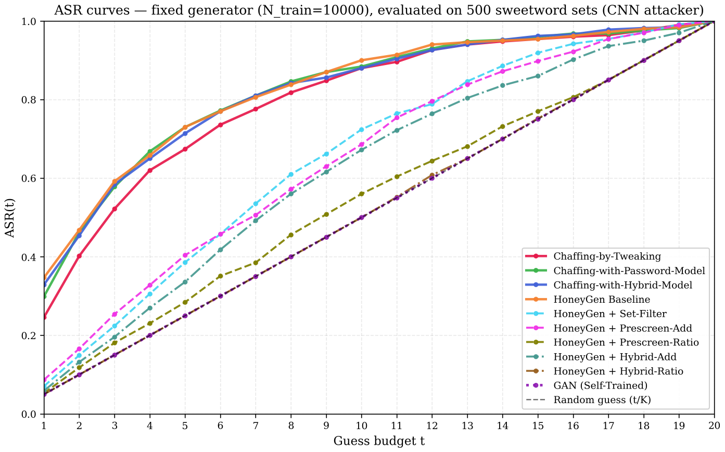
\includegraphics[width=\linewidth]{figures/cmp_N10000_e500.png}
    \caption{Test on 500 sets.}
  \end{subfigure}

  \medskip
  \begin{subfigure}{0.66\textwidth}
    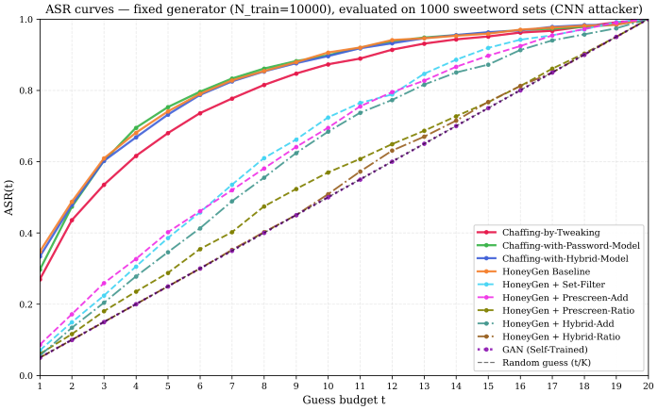
\includegraphics[width=\linewidth]{figures/cmp_N10000_e1000.png}
    \caption{Test on 1000 sets.}
  \end{subfigure}

  \medskip
  \begin{subfigure}{0.66\textwidth}
    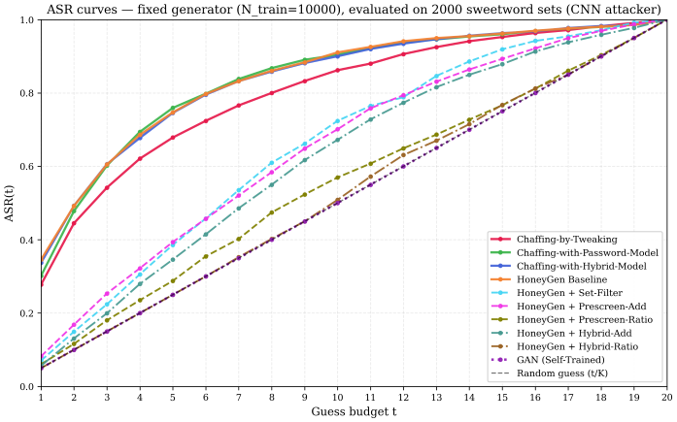
\includegraphics[width=\linewidth]{figures/cmp_N10000_e2000.png}
    \caption{Test on 2000 sets.}
  \end{subfigure}
  \caption{ASR curves under the CNN attacker at $N_{\text{train}} = 10000$
  for all ten methods, evaluated on test sets of 500, 1000, and 2000
  sweetword sets. The three panels keep the same shape and the same
  ordering of methods as the test set grows.}
  \label{fig:cmp-all}
\end{figure}

\section{The GAN Result Requires a Caveat}
\label{sec:results-gan}

% Mixed-corpus attacker figure (smaller, inline). The frequency-attacker
% results are reported in Table (tab:crossatt), not as a figure.

\begin{figure}[ht]
  \centering
  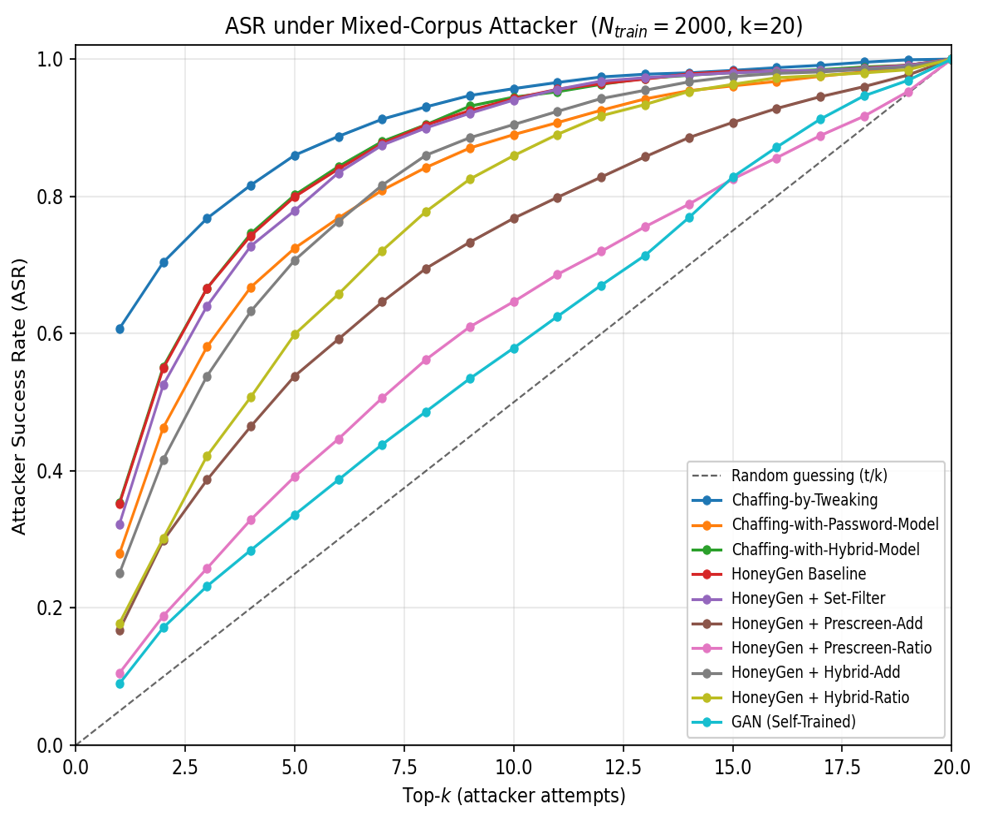
\includegraphics[width=0.72\textwidth]{figures/asr_mixed_N2000.png}
  \caption{ASR curves under the mixed-corpus attacker (trained on
  Tweak + Password-Model + HoneyGen + GAN negatives) at
  $N_{\text{train}} = 2000$, test on 2000 passwords. The GAN moves off
  the random-guessing diagonal it hugged under the single-family CNN
  attacker, and the effect strengthens with training size
  (\Cref{sec:results-gan}).}
  \label{fig:asr-mixed-2000}
\end{figure}


The GAN's reported $\mathrm{ASR}@5 = 0.872$ at $N_{\text{train}} = 10000$
(\Cref{tab:asr-master}) makes it one of the weakest methods in the
benchmark, but the reason is worth spelling out, because an attacker
that simply followed the CNN would conclude the opposite.
\Cref{tab:gan} reports two attacker strategies side by side together
with $F_{\text{rank}}$.

% ===== GAN artifact table (N_train=10000, N_eval=2000) =====
\begin{table}[t]
  \centering
  \begin{tabular}{lrrrr}
    \toprule
    \textbf{Method} & Follow-CNN & Anti-CNN & Reported & $F_{\text{rank}}$ \\
     & $\mathrm{ASR}@5$ & $\mathrm{ASR}@5$ & $\mathrm{ASR}@5$ & \\
    \midrule
    HoneyGen Baseline & 0.746 & 0.038 & 0.746 & 0.169 \\
    HoneyGen + Prescreen-Ratio & 0.341 & 0.180 & 0.341 & 0.422 \\
    HoneyGen + Hybrid-Ratio & 0.293 & 0.202 & 0.293 & 0.462 \\
    GAN (Self-Trained) & 0.025 & 0.872 & 0.872 & 0.920 \\
    \bottomrule
  \end{tabular}
  \caption{Two attacker strategies at $N_{\text{train}}=10000$:
  \emph{Follow-CNN} guesses the CNN's top-ranked candidates,
  \emph{Anti-CNN} guesses its bottom-ranked ones, and \emph{Reported}
  is the rational-attacker value of \Cref{eq:rational}. For the baseline
  and the ratio filters, Follow-CNN is the larger of the two directions
  and $F_{\text{rank}}$ sits near or above $0.4$, so the reported value
  simply follows the CNN. The GAN is the exception --- its
  $F_{\text{rank}}$ near $1$ places the real password at the bottom, so
  Follow-CNN succeeds only $2.5\%$ of the time while Anti-CNN reaches
  $87\%$. Its low Follow-CNN score is inverted distinguishability, not
  flatness.}
  \label{tab:gan}
\end{table}


For HoneyGen Baseline, following the CNN's top-ranked guesses succeeds
$74.6\%$ of the time and $F_{\text{rank}}$ is $0.169$ --- the real
password sits near the top, so the attacker just follows the CNN. For
the ratio filters both attacker directions land near the
random-guessing rate and $F_{\text{rank}}$ is close to the ideal $0.5$;
the real password is in the middle, so neither direction helps and the
sets are genuinely flat. The GAN is the exception. Following the CNN
succeeds only $2.5\%$ of the time, which taken alone would make the GAN
look like the flattest method in the benchmark, but its
$F_{\text{rank}}$ is $0.920$: the real password is ranked at or near the
bottom of almost every GAN set. A rational attacker inverts and guesses
the CNN's \emph{lowest}-scored candidates, and succeeds $87.2\%$ of the
time --- which is the value the two-sided floor of \Cref{eq:rational}
reports. A GAN trained on the oracle corpus samples from the corpus's
high-probability region, and the real password, itself a low-probability
sample, looks like an outlier the classifier confidently rejects; this
is inverted distinguishability, not flatness.

The bias is confirmed by a change of attacker. Under the
mixed-corpus attacker of \Cref{sec:method-cnn} --- trained on Tweak,
Password-Model, HoneyGen and GAN negatives together --- the GAN leaves
the random-guessing diagonal it hugged under the single-family CNN
attacker: at $N_{\text{train}} = 2000$ its $\mathrm{ASR}@5$ rises from
$0.21$ to $0.34$ (\Cref{fig:asr-mixed-2000}), and the effect grows with
training size, reaching $0.99$ at $N_{\text{train}} = 5000$, while the
filtered ratio methods shift comparatively little.
\Cref{tab:mixed} lists the per-method $\mathrm{ASR}@5$ under the two
attackers at $N_{\text{train}} = 2000$. Whether it is exposed by the
inverted CNN strategy or by a broader attacker, the GAN's apparent
flatness under a naive single-family attacker is not a property of the
sweetword sets it produces.

% ===== CNN vs Mixed attacker (N_train=2000, matches slide 15) =====
\begin{table}[t]
  \centering
  \begin{tabular}{lrr}
    \toprule
    \textbf{Method} & CNN-only $\mathrm{ASR}@5$ & Mixed-corpus $\mathrm{ASR}@5$ \\
    \midrule
    Chaffing-by-Tweaking & 0.679 & 0.860 \\
    Chaffing-with-Password-Model & 0.759 & 0.725 \\
    Chaffing-with-Hybrid-Model & 0.756 & 0.802 \\
    HoneyGen Baseline & 0.752 & 0.799 \\
    HoneyGen + Set-Filter & 0.728 & 0.779 \\
    HoneyGen + Prescreen-Add & 0.588 & 0.538 \\
    HoneyGen + Prescreen-Ratio & 0.417 & 0.392 \\
    HoneyGen + Hybrid-Add & 0.641 & 0.707 \\
    HoneyGen + Hybrid-Ratio & 0.503 & 0.599 \\
    GAN (Self-Trained) & 0.212 & 0.336 \\
    \bottomrule
  \end{tabular}
  \caption{$\mathrm{ASR}@5$ under the HoneyGen-only CNN attacker versus the
  mixed-corpus attacker (Tweak + Password-Model + HoneyGen + GAN negatives)
  at $N_{\text{train}}=2000$. The GAN moves off the near-floor value it
  reported under the CNN-only attacker ($0.21 \to 0.34$), while the
  filtered ratio methods shift comparatively little; the effect is much
  larger at $N_{\text{train}}=5000$ (\Cref{sec:results-gan}).}
  \label{tab:mixed}
\end{table}


\section{Robustness Across Attacker Class}
\label{sec:results-freq}

The filter is tuned against the CNN attacker, so we check the accepted
sets against the two robustness attackers of
\Cref{sec:method-robustness-attackers}: an independent frequency ranker
and a mixed-corpus CNN. \Cref{tab:crossatt} reports the CNN and the
frequency attacker at $N_{\text{train}} = 10000$.

% ===== Cross-attacker CNN vs Freq (N_train=10000) =====
\begin{table}[t]
  \centering
  \begin{tabular}{lrrrr}
    \toprule
    & \multicolumn{2}{c}{\textbf{CNN attacker}} & \multicolumn{2}{c}{\textbf{Freq. attacker}} \\
    \cmidrule(lr){2-3}\cmidrule(lr){4-5}
    \textbf{Method} & $\mathrm{ASR}@1$ & $\mathrm{ASR}@5$ & $\mathrm{ASR}@1$ & $\mathrm{ASR}@5$ \\
    \midrule
    Chaffing-by-Tweaking & 0.281 & 0.678 & 0.216 & 0.386 \\
    Chaffing-with-Password-Model & 0.304 & 0.755 & 0.050 & 0.250 \\
    Chaffing-with-Hybrid-Model & 0.337 & 0.743 & 0.083 & 0.319 \\
    HoneyGen Baseline & 0.346 & 0.746 & 0.084 & 0.319 \\
    HoneyGen + Set-Filter & 0.179 & 0.610 & 0.086 & 0.322 \\
    HoneyGen + Prescreen-Add & 0.144 & 0.525 & 0.050 & 0.250 \\
    HoneyGen + Prescreen-Ratio & 0.071 & 0.341 & 0.050 & 0.250 \\
    HoneyGen + Hybrid-Add & 0.141 & 0.510 & 0.068 & 0.286 \\
    HoneyGen + Hybrid-Ratio & 0.050 & 0.293 & 0.076 & 0.305 \\
        GAN (Self-Trained) & 0.745 & 0.872 & 0.225 & 0.388 \\
    \bottomrule
  \end{tabular}
  \caption{Cross-attacker comparison at $N_{\text{train}}=10000$
  (rational-attacker $\mathrm{ASR}$, \Cref{eq:rational}).
  The frequency attacker separates the methods far less sharply than the
  CNN; the filtered HoneyGen variants stay near the frequency floor. The
  GAN is distinguishable under both attackers --- most strongly by the
  CNN, which reaches $0.872$ once its ranking is inverted (the real
  password sits at the bottom), and also by the frequency attacker at
  $0.388$; it is flat under neither, as discussed in
  \Cref{sec:results-gan}.}
  \label{tab:crossatt}
\end{table}


Three points follow. First, the frequency attacker is a substantially
weaker distinguisher than the CNN: its $\mathrm{ASR}@5$ on HoneyGen
Baseline is 0.319 versus 0.746 for the CNN. This is the gap
PassFilter identified --- methods evaluated only against ranker-style
attackers report flatness numbers that overstate their security once a
learned discriminator is admitted. Second, filtering against the CNN
does not open the sets up to the frequency attacker: the filtered
variants stay near the frequency floor, so there is no security
trade-off between the two attacker classes. This absence of a trade-off
is somewhat surprising, since tuning a filter to one attacker does not
in general protect against a different one, and we do not have a proven
explanation for it. A plausible one is that the features the CNN relies
on to judge how ``real'' a candidate looks are themselves correlated
with popularity --- the common structural patterns that also drive the
frequency ranker --- so a set the CNN cannot separate tends to be one
the frequency attacker cannot separate either. We report this as an
empirical observation rather than a guarantee; whether the two attacker
classes genuinely align, or whether a trade-off appears against a
stronger ranker, is left as future work. Third, the GAN is
distinguishable to both attackers rather than flat: its frequency
$\mathrm{ASR}@5$ of 0.388 is the highest frequency value in the table,
and under the CNN a rational attacker that inverts the ranking reaches
0.872 (\Cref{sec:results-gan}). The GAN is thus caught from both
directions --- by the frequency ranker directly and by the CNN once its
anti-informative ranking is inverted.

\section{Discussion}
\label{sec:results-discussion}

The picture is consistent across training size and attacker class,
with four conclusions.

\emph{First, unfiltered honeyword generators are vulnerable to a CNN
attacker.} The four baselines report $\mathrm{ASR}@5$ around
$0.68$--$0.76$ across all three corpus sizes, about three times the
random-guessing rate, and the sophistication of the generator does not
translate into flatness.

\emph{Second, filtering restores flatness, most strongly in the ratio
variant.} The ratio filters bring $\mathrm{ASR}@5$ down to
0.341--0.293 at $N_{\text{train}} = 10000$ with $F_{\text{rank}}$
near the ideal middle, and preserve most of that reduction at smaller
sizes; the additive filters achieve a moderate reduction at a much
lower rejection cost.

\emph{Third, acceptance is a first-class requirement.} Under the
relaxed thresholds every filtered method is deployable
($>25\%$ acceptance) at every corpus size, and the recommended
configurations are the ratio filters read through the two-stage
criterion of \Cref{sec:results-cost}: the flattest methods that remain
deployable.

Fourth, the GAN's apparent success is a distributional artifact.
Following the CNN naively, the GAN looks like the flattest method, but
$F_{\text{rank}}$ far from the ideal middle value of $0.5$ ---
$0.920$, not $0$ --- shows the real password is ranked at the bottom
rather than the top, so a rational attacker who inverts the ranking
reaches $\mathrm{ASR}@5 = 0.872$ (\Cref{eq:rational}); the same bias is exposed
by the mixed-corpus attacker, and the GAN is also the most
distinguishable method under the frequency attacker. Any security claim
that treats the GAN as a strong flatness-preserving generator has to
face this data. \Cref{ch:conclusion} takes these conclusions as its
starting point.
